\subsection{Esecuzione dell'esperienza}

L'esecuzione dell'esperienza è molto semplice. Avevamo a nostra disposizione le seguenti diapositive:

\begin{itemize}
    \item{Diapositiva con fessure di larghezza nominale 160, 80, 40 e 20 micrometri.}
    \item{Diapositiva con 5 fili di spessore sconosciuto a cui abbiamo aggiunto un capello di uno dei membri del gruppo.}
    \item{Diapositiva con 2 fori di diametro ignoto.}
    \item{Diapositiva con 3 reticoli da 100, 300 e 600 fessure per millimetro.}
\end{itemize}

Le misure sono state eseguite nel seguente modo. Per ogni diapositiva, abbiamo posto sul percorso del raggio laser ogniuno degli ostacoli
presenti sulla diapositiva, uno alla volta (ovviamente :-) ). Nel fare ciò, ci siamo presi la briga di controllare, alzando ed abbassando
la diapositiva, che la figura di diffrazione fosse la più pulita possibile. Questo significa trovare il luogo della fessura che ha i bordi
migliori. Dopodiché abbiamo incollato allo schermo una striscia di carta per annotare picchi e minimi. Siccome la figura cambia a seconda
dell'ostacolo è stato fatto come segue:

\begin{itemize}
    \item{Nel caso di fili e fessure la figura di diffrazione è lineare e presenta dei massimi e minimi larghi e ``sfuocati'' con un andamento
        sinusoidale (si veda Figura \ref{fig:ff}). Abbiamo segnato sulla carta i minimi di intensità, ovvero le parti dello schermo
        che restano al buio.}
    \item{Nel caso dei fori la figura di diffrazione è un cerchio centrale con vari anelli luminosi concentrici separati da
        zone scure (minimi di intensità, si veda Figura \ref{fig:foro}). Inoltre, a parte il centro ed il primo anello,
        la figura è molto debole e difficilmente
        percepibile ad occhio nudo. Poiché la misura del primo minimo è difficoltosa a causa della larghezza dello stesso, abbiamo segnato
        l'inizio e la fine del minimo e poi mediato i valori ottenuti.}
    \item{Nel caso dei reticoli di diffrazione la figura di interferenza presenta dei picchi molto luminosi e dei minimi molto larghi
            (In realtà ci sono anche dei minimi secondari, ma sono talmente deboli da non essere percepibili. Disegno in Figura \ref{fig:ret}).
            La misura dei minimi è quindi
        esclusa, per cui abbiamo misurato la separazione tra i massimi dello stesso ordine.}
\end{itemize}

\begin{figure}[t]
    \centering
    \begin{subfigure}[b]{0.3\textwidth}
        
\includegraphics[width=\textwidth]{f1.png}
        \caption{Filo o una fessura.}
        \label{fig:ff}
    \end{subfigure}%
    ~ %add desired spacing between images, e. g. ~, \quad, \qquad etc.
      %(or a blank line to force the subfigure onto a new line)
    \begin{subfigure}[b]{0.3\textwidth}
        
\includegraphics[width=\textwidth]{f2.png}
        \caption{Foro.}
        \label{fig:foro}
    \end{subfigure}
    ~ %add desired spacing between images, e. g. ~, \quad, \qquad etc.
      %(or a blank line to force the subfigure onto a new line)
    \begin{subfigure}[b]{0.3\textwidth}
        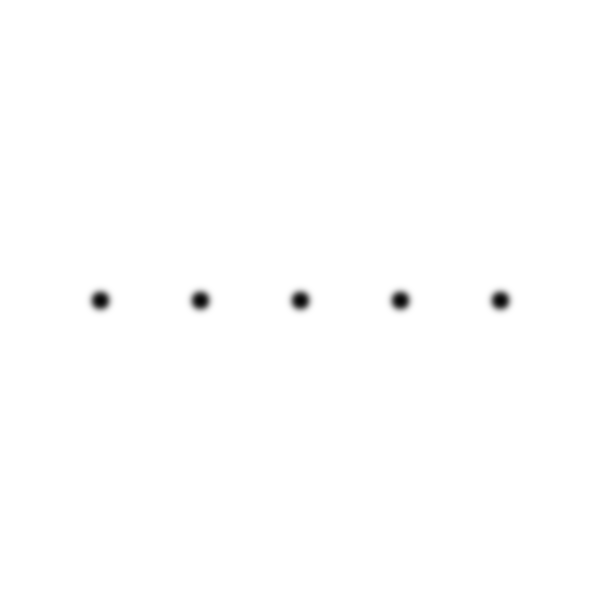
\includegraphics[width=\textwidth]{f3.png}
        \caption{Reticolo.}
        \label{fig:ret}
    \end{subfigure}
    \caption{Figure di diffrazione generate da diversi tipi di ostacoli. Notare che le aree nere sono quelle illuminate,
    mentre quelle bianche sono quelle che restano al buio.}
    \label{fig:diff}
\end{figure}
